%%%%%%%%%%%%%%%%%%%%%%%%%%%%%%%%%%%%%%%%%%%%%%%%%%%%%%%%%%%%%%%%%
% Contents: The transactions chapter
% $Id: grisbi-manuel-transactions.tex,v 0.4 2002/10/27 Daniel Cartron
% $Id: grisbi-manuel-transactions.tex, v 0.5.0 2004/06/01 Loic Breilloux
% some of its content was in tips chapter: 
% $Id: grisbi-manuel-tips.tex, v 0.4 2002/10/27 Daniel Cartron
% $Id: grisbi-manuel-transactions.tex, v 0.6.0 2011/11/17 Jean-Luc Duflot
% some of its content was in tips chapter:
% $Id: grisbi-manuel-tips.tex, v 0.5.0 2004/06/01 Loic Breilloux
% $Id: grisbi-manuel-transactions.tex, v 0.8.9 2012/04/27 Jean-Luc Duflot
% $Id: grisbi-manuel-transactions.tex, v 1.0 2014/02/12 Jean-Luc Duflot
% some of its content was in accounts chapter:
% $Id: grisbi-manuel-accounts.tex, v 0.8.9 2012/04/27 Jean-Luc Duflot
% $Id: 08-grisbi-manuel-transaction-fr.tex, v 3.0 2026/05 Dominique Brochard
%%%%%%%%%%%%%%%%%%%%%%%%%%%%%%%%%%%%%%%%%%%%%%%%%%%%%%%%%%%%%%%%%

\chapter{Buchungen\label{transactions}}
%\chapter{Account transactions\label{transactions}}
%\chapter{Opérations d'un compte\label{transactions}}

Die verschiedenen Konten, die Sie erstellen haben, enthalten Buchungen. Um die Liste der in Ihrer Kontendatei gespeicherten Konten anzuzeigen, verwenden Sie die Informationsleiste oder das Navigationsbereich (siehe das Kapitel \vref{home}, \menus{Startseite} und den Abschnitt \vref{accounts-list}, \menus{Liste der Konten}).
%The various accounts you have created contain transactions. To view the list of accounts stored in your accounts file, use the information bar or the navigation panel (see the \vref{home}, \menus{Home} chapter and the \vref{accounts-list}, \menus{Account List} section).
%Les différents comptes que vous avez créés contiennent les opérations. Pour afficher la liste des comptes enregistrés dans votre fichier de comptes, utilisez la barre d'information ou le panneau de navigation (voir le chapitre \vref{home}, \menus{Accueil} et la section \vref{accounts-list}, \menus{Liste des comptes}).

Um die Transaktionen eines Kontos anzuzeigen, wählen Sie dieses Konto aus der Liste aus: Standardmäßig wird die Registerkarte \menus{Buchungen} angezeigt. Sie enthält vier Hauptbereiche:
%To view the transactions for an account, select that account from the list: the \menus{Transactions} tab will appear by default. It contains four main sections:
%Pour afficher les opérations d'un compte, sélectionnez ce compte dans la liste: l'onglet \menus{Opérations} s'affiche par défaut. Il possède quatre éléments principaux:

\begin{enumerate}
	\item Werkzeugliste;
	%\item the toolbar;
	%\item la barre d'outils;
	\item Buchungsliste;
	%\item the list of transactions;
	%\item la liste des opérations;
	\item Buchungsformular
	%\item the transaction/scheduled form;
	%\item le formulaire de saisie des opérations;
	\item Abgestimmter saldo.
	%\item the \indexword{reconciled balance}\index{balance!reconciled}.
	%\item le \indexword{solde pointé}\index{solde!pointé}.
\end{enumerate}

% espace avant Attention ou Note: 5 mm
\vspacepdf{3mm}
\Note{}: Wenn Sie noch nie einen Abgleich durchgeführt haben, also keine Abstimmungen vorgenommen haben, kann Grisbi keinen abgeglichenen Saldo berechnen oder anzeigen.
%\Note{}: if you have never carried out a reconciliation – i.e. you have not performed any reconciliation entries – Grisbi cannot calculate or display a reconciled balance.
%\Note{}: si vous n'avez jamais fait de rapprochement, donc pas de pointages, Grisbi ne peut ni calculer ni afficher de solde rapproché.


\section{Werkzeugliste\label{transactions-functions}}
%\section{Toolbar\label{transactions-functions}}
%\section{Barre d'outils\label{transactions-functions}}

Die Werkzeugleiste befindet sich oben im Detailbereich und bietet folgende Funktionen:
%The toolbar is located at the top of the details panel and offers the following functions:
%La barre d'outils est présente en haut du panneau des détails et présente les fonctions suivantes:

\begin{itemize}
	\item \menus{Buchung erstellen}: springt zum Ende der Buchungsliste und öffnet ein leeres Buchungsformular;
	%\item \menus{New transaction}: goes to the end of the list of transactions and opens a blank entry form;
	%\item \menus{Nouvelle Opération}: va à la fin de la liste des opérations et ouvre le formulaire de saisie vierge;
	\item \menus{Löschen}: löscht die ausgewählte Buchung;
	%\item \menus{Delete}: deletes the selected transaction;
	%\item \menus{Supprimer}: supprime l'opération sélectionnée;
	\item \menus{Bearbeiten}: Öffnet das Buchungsformular für den ausgewählten Buchung und ermöglicht dessen Bearbeitung;
	%\item \menus{Edit}: opens the input form for the selected transaction and allows you to edit it;
	%\item \menus{Éditer}: ouvre le formulaire de saisie pour l'opération sélectionnée et permet de la modifier;
	\item \menus{Abstimmen}: Öffnet die Abstimmungsseite für das ausgewählte Konto (siehe Abschnitt \vref{reconciliation}, \menus{Bankabstimmung});
	%\item \menus{Reconcile}: opens the reconciliation page for the selected account (see the section \vref{reconciliation}, \menus{Bank reconciliation});
	%\item \menus{Rapprocher}: ouvre la page de rapprochement du compte sélectionné (voir le chapitre \vref{reconciliation}, \menus{Rapprochement bancaire});
	\item \menus{Drucken}: Öffnet das Fenster zur Auswahl des Druckers und seiner Optionen;
	%\item \menus{Print}: opens the window for selecting the printer and its options;
	%\item \menus{Imprimer}: ouvre la fenêtre de sélection de l'imprimante et de ses options;
	\item \menus{Ansicht}: Öffnet ein Dropdown-Menü; Sie können aus vier Optionen die \indexword{Ansicht der Buchungen}\index{Ansicht!Buchungen} auswählen:
	%\item \menus{View}: opens a drop-down menu; you can choose the \indexword{view of transactions}\index{view!transactions} from four options:
	%\item \menus{Affichage}: ouvre un menu déroulant; vous pouvez choisir l'\indexword{affichage des opérations}\index{affichage!opérations} parmi quatre possibilités:
		\begin{itemize} 
			\item \menus{Einzeilig},
			%\item \menus{Simple view},
			%\item \menus{Vue simple},
			\item \menus{Zweizeilig},
			%\item \menus{Two lines view},
			%\item \menus{Mode \frquote{deux lignes}},
			\item menus{Dreizeilig},
			%\item \menus{Three lines view},
			%\item \menus{Mode \frquote{trois lignes}},
			\item \menus{Vollständig},
			%\item \menus{Complete view},
			%\item \menus{Vue complète},
			\item[] \hspace{-15pt} sowie:
			%\item[] \hspace{-15pt} as well as:
			%\item[] \hspace{-15pt} ainsi que:
			\item die Anzeige oder Nichtanzeige der \indexword{abgestimmte Buchungen}\index{Anzeige!abgestimmte Buchungen},
			%\item whether or not to show \indexword{reconciled operations}\index{show!reconciled operations},
			%\item l'affichage ou non des \indexword{opérations rapprochées}\index{affichage!opérations rapprochées},
			\item ob die erstellten Archive angezeigt werden sollen oder nicht \indexword{archivezeilen}\index{anzeige!archivezeilen} (\vref{datamanagement-archive-display}),
			%\item whether or not to show the \indexword{archives lines}\index{display!archives lines} (\vref{datamanagement-archive-display}),
			%\item l'affichage ou non des \indexword{lignes d'archives}\index{affichage!lignes d'archives} (\vref{datamanagement-archive-display}),
		\end{itemize}
		\vspacepdf{2mm}
	\Note{}: Die Optionen im Menü \menus{Ansicht} wirken sich standardmäßig auf die Darstellung aller Konten aus. Möglicherweise bevorzugen Sie für jedes Konto eine andere Darstellung; dies kann im Menü \menus{Bearbeiten – Einstellungen – Buchungen – Einstellungen} konfiguriert werden (siehe Abschnitt \vref{setup-operations-list-differentiation}, \menus{Konto-Differenzierung}).
	%\Note{}: the options in the \menus{View} menu affect the display of all accounts by default. You may prefer a different display for each account; this can be configured in the \menus{Edit - Preferences - Transactions - List Behaviour} menu (see the section \vref{setup-operations-list-differentiation}, \menus{Account Differentiation}).
	%\Note{}: les options du menu \menus{Affichage} influent par défaut sur l'affichage de tous les comptes. Vous pouvez préférer un affichage différent pour chaque compte, cela est configurable dans le menu \menus{Éditer - Préférences - Opérations - Comportement de la liste} (voir le paragraphe \vref{setup-operations-list-differenciation}, \menus{Différenciation des comptes}).	
	\item ein Feld \menus{Buchungen suchen}, das mindestens drei Zeichen enthalten muss,
	%\item a \menus{Search} box, which must contain at least three characters,
	%\item un champ \menus{Rechercher}, à remplir avec trois caractères minimum, 
	\item eine Dropdown-Liste auf der rechten Seite, mit der Sie die angezeigten Vorgänge nach folgenden Kriterien filtern können:
	%\item a drop-down list on the right that allows you to filter the displayed operations by:
	%\item une liste déroulante associée, à droite, permettant de filtrer les opérations affichées selon:
		\begin{itemize} 
			\item der \menus{Empfänger Name},
			%\item the \menus{Payee name},
			%\item le \menus{Nom du tiers},
			\item der \menus{Notiz},
			%\item the \menus{Note},
			%\item la \menus{Remarque},
			\item der \menus{Empfänger und Notiz} (standardmäßig ausgewählt),
			%\item the \menus{Payee and note} (selected by default),
			%\item les \menus{Tiers et remarque} (sélectionné par défaut),
			\item der \menus{Gruppe},
			%\item the \menus{Budgetary line},
			%\item l'\menus{Imputation budgétaire},
			\item der \menus{Kategorie}.
			%\item the \menus{Category}.
			%\item la \menus{Catégorie}.
	\end{itemize}
	\vspacepdf{2mm}
	\Note{}: Die Suche erfolgt ohne Berücksichtigung der Groß-/Kleinschreibung und muss mindestens drei (3) alphanumerische Zeichen enthalten; es werden nur die übereinstimmenden Vorgänge in der Vorgangsliste angezeigt. Die Suche wird AUSSCHLIESSLICH auf die angezeigten Vorgänge angewendet (beachten Sie, ob die \indexword{abgestimmte Buchungen}\index{Anzeige!abgestimmte Buchungen} angezeigt werden) und umfasst nicht die Archive.
	%\Note{}: the search is case-insensitive and must include at least three (3) alphanumeric characters; it displays only the matching operations in the list of operations. The search is performed ONLY on the displayed operations (note whether or not the \indexword{reconciled operations}\index{show!reconciled operations} are shown) and does not include the archives.
	%\Note{}: la recherche est insensible à la casse et doit se faire avec un minimum de trois (3) caractères alpha-numériques; elle affiche uniquement toutes les opérations correspondantes dans la liste des opérations. La recherche ne se fait QUE sur les opérations affichées (attention à l'affichage ou non des \indexword{opérations rapprochées}\index{affichage!opérations rapprochées}) et ne concerne pas les archives.
	
	
	\item ein Schnellsuchfeld und eine Dropdown-Liste, mit denen Sie nach folgenden Kriterien filtern können:
	%\item a quick search box and a drop-down list allowing you to filter by:
	%\item un champ de recherche rapide et une liste déroulante permettant de filtrer selon:
		\begin{itemize} 
			\item \menus{Empfänger Name},
			%\item \menus{Payee name},
			%\item le \menus{Nom du tiers},
			\item \menus{Notiz},
			%\item \menus{Note},
			%\item la \menus{remarque},
			\item \menus{Empfänger und Notiz},
			%\item \menus{Payee and note},
			%\item les \menus{Tiers et remarque},
			\item \menus{Gruppe},
			%\item \menus{Budgetary line},
			%\item l'\menus{Imputation budgétaire},
			\item \menus{Kategorie}.
			%\menus{Category}.
			%\item la \menus{Catégorie}.
		\end{itemize}
\end{itemize}


\section{Liste der Buchungen\label{transactions-list}}
%\section{List of transactions\label{transactions-list}}
%\section{Liste des opérations\label{transactions-list}}


\subsection{Beschreibung\label{transactions-list-description}}
%\subsection{Description\label{transactions-list-description}}
%\subsection{Description\label{transactions-list-description}}

Die Liste der Buchungen wird im Bereich details\refimage{transactions-list-img} unterhalb der Werkzeugleiste angezeigt.
%The list of transactions is displayed in the details panel\refimage{transactions-list-img} below the toolbar.
%La liste des opérations s'affiche dans le panneau des détails\refimage{transactions-list-img} sous la barre d'outils.

% image centrée 
\begin{figure}[ht]
	\begin{center}
	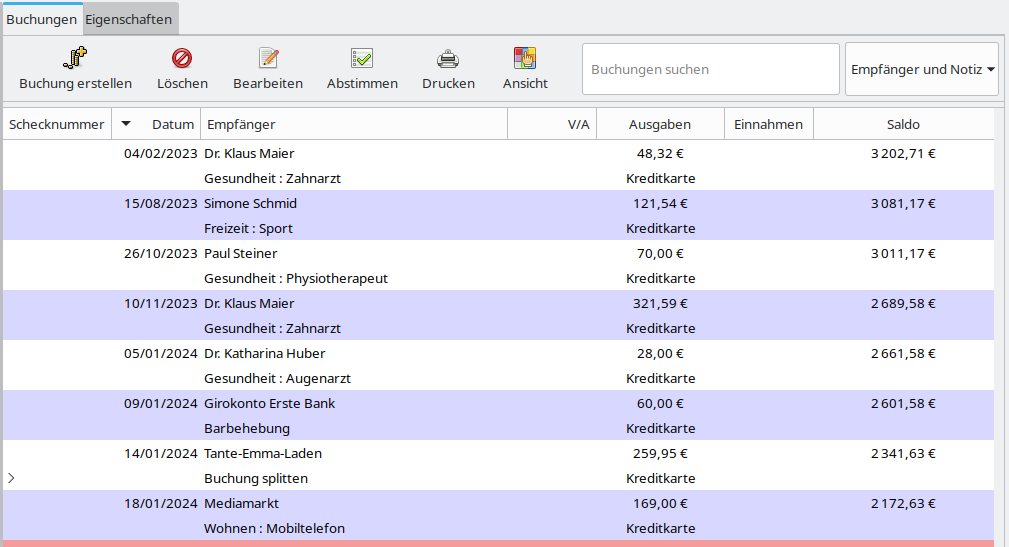
\includegraphics[width=0.95\textwidth]{image/screenshot/transactions_list}
	\end{center}
	\caption{Liste der Buchungen}
	%\caption{List of transactions}
	%\caption{Liste des opérations}
	\label{transactions-list-img}
\end{figure}
% image centrée 


Oben wird die Spaltenkopfzeile angezeigt. Sie können \indexword{eine Spalte verbreitern oder verengen}\index{Spalte!Breite}, indem Sie auf die Trennlinie zwischen zwei Spalten klicken und diese ziehen. Um die Spalten wieder auf ihre Standardbreite zurückzusetzen, wählen Sie \menus{Ansicht – Spaltenbreite zurücksetzen} aus der Menüleiste.
%The column header bar is displayed at the top. You can \indexword{widen or narrow a column}\index{column!width} by clicking on the separator between two columns and dragging it. To restore the columns to their default width, select \menus{View - Reset the column width} from the menu bar.
%Elle affiche en haut la barre des libellés des colonnes. Vous pouvez \indexword{élargir ou rétrécir une colonne}\index{colonne!largeur} en cliquant sur le séparateur entre deux colonnes et en le déplaçant. Pour rétablir la largeur des colonnes à leur valeur par défaut, sélectionnez dans la barre de menu \menus{Affichage - Réinitialiser la largeur des colonnes}.

Sie können mit dem Mausrad oder durch Ziehen der vertikalen Bildlaufleiste in der Liste der Buchungen nach oben oder unten scrollen. Um nach links oder rechts zu scrollen, ziehen Sie die horizontale Bildlaufleiste mit der Maus.
%You can scroll the list of transactions up or down using the mouse wheel, or by dragging the vertical scroll bar. To scroll left or right, use the mouse to drag the horizontal scroll bar.
%Vous pouvez déplacer la liste des opérations vers le haut ou vers le bas avec la molette de la souris, ou bien avec la souris et l'ascenseur vertical. Le déplacement vers la gauche ou la droite se fait avec la souris et l'ascenseur horizontal.

Sie können wählen, ob Folgendes angezeigt werden soll oder nicht:
%You can choose whether or not to display:
%Vous pouvez choisir d'afficher ou non:
\begin{itemize}
	\item die \indexword{Abgestimmte Buchungen}\index{anzeigen!Abgestimmte Buchungen} durch Auswahl von:
	%\item the \indexword{reconciled transactions}\index{display!reconciled transactions} by selecting:
	%\item les \indexword{opérations rapprochées}\index{affichage!opérations rapprochées} en sélectionnant:
		\begin{itemize}
			\item in der Menüleiste \menus{Ansicht - Abgestimmte Buchungen anzeigen} (\keys{Alt+R}) (siehe Abschnitt \vref{home-menus-display}),
			%\item in the menu bar \menus{View - Show reconciled transactions} (\keys{Alt+R}) (see the section \vref{home-menus-display}),
			%\item dans la barre de menu \menus{Affichage - Montrer les opérations rapprochées} (\keys{Alt+R}) (voir la section \vref{home-menus-display}),
			\item in der Werkzeugleiste \menus{Ansicht - Abgestimmte Buchungen anzeigen} (siehe Abschnitt \vref{transactions-functions}),
			%\item in the toolbar \menus{View - Show reconciled Transactions} (section \vref{transactions-functions});
			%\item dans la barre d'outils \menus{Affichage - Montrer les opérations rapprochées} (section \vref{transactions-functions});
		\end{itemize} 
	\item die \indexword{Archivzeilen}\index{anzeige!Archivzeilen} (siehe Abschnitt \menus{Anzeige des Archivs} \vref{datamanagement-archive-display}):
	%\item the \indexword{lines archives}\index{display!lines archives} (see the section \menus{Archives display} \vref{datamanagement-archive-display}):
	%\item les \indexword{lignes d'archives}\index{affichage!lignes d'archives} (voir la section \menus{Affichage des archives} \vref{datamanagement-archive-display}):
		\begin{itemize}
			\item in der Menüleiste \menus{Ansicht - Erstellte Archive anzeigen} (\keys{Alt+L}) (see the section \vref{home-menus-display}),
			%\item in the menu bar \menus{View - Show lines archives} (\keys{Alt+L}) (see the section \vref{home-menus-display}),
			%\item dans la barre de menu \menus{Affichage - Montrer les lignes d'archives} (\keys{Alt+L}) (voir la section \vref{home-menus-display}),
			\item in der Werkzeugleiste \menus{Ansicht - Erstellte Archive anzeigen} (section \vref{transactions-functions}).
			%\item in the toolbar \menus{View - Show lines archives} (section \vref{transactions-functions}).
			%\item dans la barre d'outils \menus{Affichage - Montrer les lignes d'archives} (section \vref{transactions-functions}).
		\end{itemize}
\end{itemize}

\vspacepdf{3mm}
Aus Sicht der Grisbi-Datenbank besteht ein Buchung aus seinen \indexword{Informationsfeldern}\index{Informationsfeld!Definition}. Die Informationsfelder jedes Buchung werden in den verschiedenen \indexword{Zellen}\index{Zelle!Informationsfeld} angezeigt, die durch den Schnittpunkt von Zeilen und Spalten definiert sind. Es können maximal vier Zeilen und sieben Spalten vorhanden sein, was ein Maximum von achtundzwanzig Informationsfeldern für jeden Buchung ergibt.
%From the perspective of the Grisbi database, a transaction consists of its \indexword{information fields}\index{information field!definition}. The information fields for each transaction are displayed in the various \indexword{cells}\index{cell!information field} defined by the intersection of rows and columns. There can be a maximum of four rows and seven columns, which defines a maximum of twenty-eight information fields for each transaction.
%Du point de vue de la base de données de Grisbi, une opération est constituée de ses \indexword{champs d'information}\index{champ d'information!définition}. Les champs d'information de chaque opération s'affichent dans les différentes \indexword{cellules}\index{cellule!champ d'information} définies par l'intersection des lignes et des colonnes. Il ne peut y avoir au maximum que quatre lignes et sept colonnes, ce qui définit un maximum de vingt-huit champs d'information pour chaque opération.

Jede Buchung kann je nach ausgewähltem Anzeigemodus über 1, 2, 3 oder 4 Zeilen angezeigt werden (siehe Abschnitt \vref{home-menus-display}, das Menü \menus{Ansicht} in der Menüleiste oder die Funktion \menus{Ansicht} im Abschnitt \vref{transactions-functions}, \menus{Werkzeugleiste}). Die aktuelle Anzeige wird durch ein Häkchen gekennzeichnet.
%Each transaction can be displayed over 1, 2, 3 or 4 lines, depending on the selected display mode (see the \vref{home-menus-display} section, the \menus{View} menu in the menu bar, or the \menus{View} function in the \vref{transactions-functions}, \menus{Toolbar} section). The current display is indicated by a tick.
%Chaque opération peut être affichée sur 1, 2, 3 ou 4 lignes, suivant le mode d'affichage sélectionné (voir la section \vref{home-menus-display}, menu \menus{Affichage} dans la barre de menu ou la fonction \menus{Affichage} dans la section \vref{transactions-functions}, \menus{Barre d'outils}). L'affichage courant y est indiqué par une coche.

Sie können den Inhalt dieser Zeilen sowie das Speichern der Anzeigeeinstellungen auch für jedes Konto einzeln im Menü \menus{Bearbeiten - Einstellungen - Buchungen} konfigurieren (siehe die Abschnitte \vref{setup-operations-list}, \menus{Einstellungen} und \vref{setup-operations-cells}, \menus{Buchungsübersicht Zellen}).
%You can also configure the content of these lines, as well as the saving of display settings, individually for each account, in the \menus{Edit - Preferences - Transactions} (see the sections \vref{setup-operations-list}, \menus{List behaviour} and \vref{setup-operations-cells}, \menus{Transactions list cells}).
%Vous pouvez aussi configurer le contenu de ces lignes, ainsi que la mémorisation des réglages de l'affichage, individuellement pour chaque compte, dans le menu \menus{Éditer - Préférences - Opérations} (voir les sections \vref{setup-operations-list}, \menus{Comportement de la liste} et \vref{setup-operations-cells}, \menus{Cellules de la liste des opérations}).

Die \indexword{Bezeichnung einer Spalte}\index{Spalte!Bezeichnung} ist immer der Name des Informationsfeldes, das in der ersten Zeile der Buchungen angezeigt wird.
%The \indexword{column label}\index{column!label} is always the name of the information field displayed in the first row of the transactions.
%Le \indexword{libellé d'une colonne}\index{colonne!libellé} est toujours le nom du champ d'information affiché dans la première ligne des opérations.


Um die Lesbarkeit der Anzeige zu gewährleisten, zeigt Grisbi keine Rahmen um Zellen, Spalten, Zeilen und Buchungen an, sondern wechselt in jeder Zeile zwischen einem \fboxsep=3pt{\colorbox[RGB]{215,215,255}{violetter Hintergrund}} und Weiß.
%To improve the readability of the display, Grisbi does not show any borders around cells, columns, rows or transactions, but instead uses alternating colours of  \fboxsep=3pt{\colorbox[RGB]{215,215,255}{purple background}} and white for each line.
%Pour des raisons de lisibilité de l'affichage, Grisbi n'affiche aucune bordure aux cellules, colonnes, lignes et opérations, mais présente une alternance de couleurs de  \fboxsep=3pt{\colorbox[RGB]{215,215,255}{fond violet}} et blanc à chaque ligne.

\subsection{Informations- und Eingabefelder\label{transactions-list-fields}}
%\subsection{Information and input fields\label{transactions-list-fields}}
%\subsection{Champs d'information et de saisie\label{transactions-list-fields}}

Grisbi kann für jede Buchung eine vollständige Liste von Informations- und Eingabefeldern\index{Informationsfelder} \index{Eingabefelder} verwalten, die wie folgt lauten:
%Grisbi can manage, for each transaction, a complete list of information fields and input fields\index{information fields}\index{input fields}, which are as follows:
%Grisbi sait gérer, pour chaque opération, une liste complète de champs d'information et de saisie\index{champs d'information}\index{champs de saisie}, qui sont les suivants: